\chapter{Conclusion and Thesis Research Questions}
\label{ch:conclusion}

After examination of the literature, it has become possible to draw a conclusion on the state-of-the-art of the research field, and therefore the direction and content of the proposed research. In this chapter, firstly an exposition of the identified knowledge gaps in both literature and practical engineering will be given. This will be supported by an overview of methods that can be used for carrying out the work in the research. From the knowledge gap, a main research question with supporting subquestions for the subsequent research will be derived. Lastly, a preliminary work breakdown and Gannt chart of the thesis work will be presented.

\section{Conclusion on Literature and Knowledge Gap}
In the preceding chapters, the width and depth of the research field was surveyed. The objective of this survey was to determine interesting avenues for further research, and to find promising methodology to be used in that research. \\

Firstly, the gaps in the knowledge and current capabilities will be addressed. In \autoref{ch:population}, it was found that the current completeness of asteroid surveys is highly incomplete; asteroids smaller than the 140m cut-off for PHA-status provide significant threat to human life and possessions, and a large fraction of the population has so far gone unidentified. Relating to this, \autoref{ch:surveys} provided an overview of current efforts to catalogue the asteroid population. Here, it was shown that although very large telescopes are being built and operated from Earth, they suffer from significant drawbacks that prevent them from effectively identifying a large portion of the population of asteroids at any but the last moments before impact. Ideally, plenty of advance warning should be given to defend the Earth against an asteroid, rather than only evacuating the area of impact. Space-based surveys provide a good avenue of research to improve this, and the results from e.g. NEOWISE and NEOSSat are promising. In \autoref{ch:imageprocessing}, the issues relating to the processing of the vast amounts of data produced by a sky survey were discussed. The need for automatic processing of large amounts of data has affected all fields of technical research, and space engineering is no exception. Additionally, the capabilities and techniques for automatically processing a sky image into a useful dataset were showcased. It is apparent that this field is at a very advanced level, and provides no applicable research objective. The researched techniques and the knowledge of how the methods perform are still useful, and provide good indicators of how to simulate and handle the data later. Conclusively, as was shown in \autoref{ch:trajectory}, the methods for actually determining the trajectory of a target from a series of observations are limited. Especially during short or low-quality observations, methods are not suited to processing the enormous amounts of data of an all-sky mission effectively. Therefore, the proposed research is to examine improving autonomous trajectory and impact hazard determination by a space-based telescope.\\

To carry out this research, methods were found in the literature which can be used. As the general plan, which will be laid out in \autoref{sec:plan}, shows, the idea is to simulate optical observations, process these, and develop impact hazard determination techniques for these observations. The methods for simulating the images will be based on the information on the asteroid population and properties from \autoref{ch:population}, and the knowledge of optical systems included in \autoref{ch:optical}. The image processing algorithms are discussed in \autoref{ch:imageprocessing}, although these are at a sufficiently advanced level that they are not of particular interest beyond their effect on image quality. Lastly, the techniques proposed for testing are those detailed in \autoref{ch:trajectory}: A method based on a numerical approach using the method of very short arcs, a control system approach based on the use of an extended Kalman filter, and lastly an application of dense or recurring neural networks. From assessment of literature and comparison with non-space applications of trajectory determination, it was found that these methods provide the best options for examination. The goal of this assessment is to discover if and how these methods can be used in future surveys, and what level of efficacy can be expected. 


\section{Thesis Research Questions}
With the target knowledge gap identified, and the background knowledge set, the research question will be defined as: \\

\begin{changemargin}{1cm}{1cm}
\begin{center}
\textit{\large{To what extent can impact-hazardous targets be identified through optical observations by a space system placed strategically in the solar system?}}
\end{center}
\end{changemargin}
\vspace{0.5cm}

A breakdown of the components of the question:
\begin{itemize}
\item \textbf{To what extent can… be identified}: Realistically, it will not be possible to determine the exact impact chance of all (or perhaps any) targets. However, identification of targets for further research or monitoring would be very valuable, as other observational resources can be used to track the targets more accurately.
\item \textbf{Impact-hazardous targets}: It is desirable to avoid the term “potentially hazardous asteroid”, as it already has a definition. As the problem concerns asteroids impacting Earth, it makes logical sense to see if targets that present an impact hazard can be identified. This hazard is not just a determination of the orbit; it consists of a product of impact energy (i.e. mass/size), impact probability and possibly time to impact.
\item \textbf{Optical observations by a space system}: It is not necessary to define this further, as it is an opening for this c.q. further research. The important ramification of this specification is that the space system is capable of doing the identification: Mostly, downlinking vast amounts of images to Earth for processing or analysis by humans would make the results of the research less useful: those techniques exist, but they suffer from capacity problems. This links in well with the first point, the identification information obtained by the system should be useful itself.
\item \textbf{Placed strategically in the solar system}: As measurements are taken from space, the positioning of the satellite can be examined. This would be a later stage of research, moving towards a more complete system. It is not the intention to conduct a full orbit analysis, but broad categories (e.g. Earth-Sun Lagrange points, co-orbital with Earth, co-orbital with Venus, situated in the asteroid belt) should be easy to examine once the simulations are up and running. This is however not seen as crucial in answering the question.
\end{itemize}

\renewcommand{\labelenumii}{\theenumii}
\renewcommand{\theenumii}{\theenumi.\arabic{enumii}.}
\vspace{0.3cm}
From the main questions, a set of subquestions are derived which are used to set up the work breakdown:

\begin{enumerate}
    \item How can optical obsercations of NEA's by a space system be accurately modeled?
    \begin{enumerate}
        \item What model should be used for the population of NEA's?
        \item How can the camera system be modeled?
        \item How can the simulation be verified and validated?
    \end{enumerate}
    \item How can the optical observations be processed into angular observations?
    \begin{enumerate}
        \item How precise are the methods based on correlation or analytical function fitting?
        \item Is it possible to obtain a better result using a CNN?
        \item What other information related to the impact hazard can be derived from the optical observation?
    \end{enumerate}
    \item To what extent can impact hazard be determined from these observations?
    \begin{enumerate}
        \item How can a system based on estimating and numerically searching the parameter space be implemented?
        \item How can a system based on a Kalman filter be implemented?
        \item How can a system based on an artificial neural network be implemented?
    \end{enumerate}
    \item What is the effect of strategic placement of the system on its performance?
\end{enumerate}

\section{Project Plan}
\label{sec:plan}
Before commencing the research, a planning is made to facilitate finishing the work in a timely manner. The planning is based on the TU Delft Thesis Procedure (\cite{thesisprocedure}). Firstly, an overview of all planned periods of the work is given, supplemented by national and planned holidays and contingency time. This is used to estimate the full timeframe of the project. From here, dates for the milestones are defined. Then, a work breakdown is given, and these are combined into a Gannt chart. 

\subsection{Time planning}
\autoref{tab:planning} shows the preliminary time estimate for the thesis work, culminating in a defence around the last week of January 2022. Note that this planning was made on the assumption that restrictions due to Covid-19 will be lifted around the summer of 2021. In case of unforeseen developments in this area, no claims will be made about the validity of this planning, but a new one will be developed based on best insight at the time.

\begin{table}[htbp]
\centering
\caption{Thesis timeframe planning.}
\label{tab:planning}
\begin{tabular}{llll}
\textbf{Topic}       & \textbf{Date} & \textbf{Weeks} & \textbf{Milestone}               \\ \hline \vspace{0.25cm}
Start to Kick-off    & 19/04 - 30/04 & 2              & 29/04: Kick-off Meeting           \\ \vspace{0.25cm}
Kick-off to Mid-term & 03/05 - 15/10 & 16             & 14/10: Mid-term Review            \\ \vspace{0.25cm}
Mid-term to Draft    & 18/10 - 10/12 & 6              & 10/12: Draft Thesis              \\ \vspace{0.25cm}
Draft to Green Light & 13/12 - 24/12 & 2              & 23/12: Green Light Meeting \\ \vspace{0.25cm}
Green Light to Final & 27/12 - 14/01 & 2              & 14/01: Final Thesis              \\ \vspace{0.25cm}
Final to Defence     & 17/01 - 28/01 & 2              & 28/01: Defence                   \\ \vspace{0.25cm}
Summer Holiday    & 15/07 - 28/07 & 2              & -                                \\ \vspace{0.25cm}
Study Tour       & 16/08 - 05/09 & 3              & -                                \\ \vspace{0.25cm}
Holidays Q4          & -             & 1              & -                                \\ \vspace{0.25cm}
Christmas Break      & 25/12 - 09/01 & 2              & -                                \\ \vspace{0.25cm}
Contingency          & -             & 3              & -                                \\ \hline \vspace{0.25cm}
Total                & 19/04 - 28/01 & 41             & -                               
\end{tabular}
\end{table}
\newpage
\subsection{Work Breakdown}
Following is a preliminary work breakdown based on the previously established subquestions. Included are some thoughts or elements to keep in mind when starting the components.
\begin{enumerate}
    \item Determination of mathematical foundations:
    \begin{itemize}
        \item Before working out methods or writing code, the mathematical basis for the various methods will need to be defined.
        \item This is especially important for the ANN-based solutions, as the shape of the inputs can be elemental in determining their structure.
    \end{itemize}
    \item Establishing trajectory determination methods:
    \begin{itemize}
        \item Before creating the simulation software, the methods should be defined in more detail.
        \item This order allows more time to think about the important aspects (i.e. the methods) over the simulation software.
        \item Care should be taken not to make the simulation fit the methods.
    \end{itemize}
    \item Creation of observation simulation:
    \begin{itemize}
        \item From the chapters in this review, it is known how to construct a simulation of how a satellite would observe a target.
        \item The software should be capable of producing a large amount of data, potentially for training the ANN, as well as evaluating it.
        \item Initially, only sets of angular measurements and accompanying uncertainties will be used; the further processing of optical measurements can be added later. This allows more time to resolve problems.
        \item Brightness of the target can be included as an additional parameter.
    \end{itemize}
    \item Creation of threat assessment simulation:
    \begin{itemize}
        \item The working of this simulation will provide answers to most of the questions. Therefore it is the integral part of the research work.
        \item Note that the problem is not to determine the orbit of the target as accurately as possible; the problem is to assess the risk the target poses to Earth.
        \item This step might require iteration with previous steps, depending on outcome.
        \item It should be judged early whether the code needs to be parallelizable through e.g. CUDA, should a large number of simulations be desirable.
        \item Experimentation with regards to the position of the satellite can be carried out.
    \end{itemize}
    \item Verification and validation
    \begin{itemize}
        \item Arguably the toughest topic, and the most important one. So far a solid conclusion has not been found as to the best method for verifying and validating the solution.
        \item Some ideas include tests on real-world data or using other simulation software that is freely available.
    \end{itemize}
    \item Evaluate and conclude
    \begin{itemize}
        \item Results of the simulations should be placed in context, and conclusions drawn on what would be the best suited method for this problem.
        \item To assess the feasibility of the suggested methods, they should be compared to existing surveys and background risk.
        \item Other factors such as computational complexity or time needed to image a target should be considered as well, thereby placing the research in context.
    \end{itemize}
\end{enumerate}

\newpage

\subsection{Gannt Chart}
\begin{figure}[h!]
    \centering
    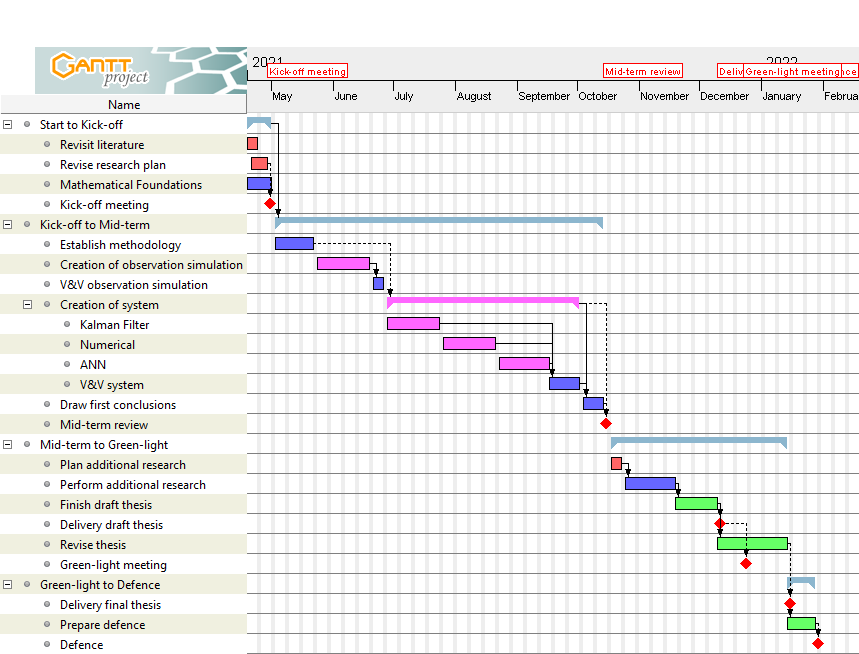
\includegraphics[width=1.0\textwidth]{images/exportportrait.png}
    \caption{Gannt chart for the thesis work. Shown in red is literature research work, blue is theoretical research work and pink the programming work. Milestones are indicated as red diamonds. Each rectangle represents a week.}
    \label{fig:gannt}
\end{figure}